\documentclass[a4paper, 11pt]{article}
\usepackage{amsmath}
\usepackage{graphicx}
\usepackage{geometry}
\usepackage{listings}
\usepackage[colorlinks,linkcolor=red]{hyperref}
\geometry{scale=0.8}

\title{	
\normalfont \normalsize
\textsc{School of Data and Computer Science, Sun Yat-sen University} \\ [25pt] %textsc small capital letters
\rule{\textwidth}{0.5pt} \\[0.4cm] % Thin top horizontal rule
\huge  E2 15-Puzzle Problem (IDA*)\\ % The assignment title
\rule{\textwidth}{2pt} \\[0.5cm] % Thick bottom horizontal rule
\author{192 Yikun Liang}
\date{\normalsize\today}
}

\begin{document}
\maketitle
\tableofcontents
\newpage

\section{IDA* Algorithm}
\subsection{Description}
Iterative deepening A* (IDA*) was first described by Richard Korf in 1985, which is a graph traversal and path search algorithm that can find the shortest path between a designated start node and any member of a set of goal nodes in a weighted graph.

It is a variant of \textbf{iterative deepening depth-first search} that borrows the idea to use a heuristic function to evaluate the remaining cost to get to the goal from the \textbf{A* search algorithm}.

Since it is a depth-first search algorithm, its memory usage is lower than in A*, but unlike ordinary iterative deepening search, it concentrates on exploring the most promising nodes and thus does not go to the same depth everywhere in the search tree.

\textbf{Iterative-deepening-A* works as follows:} at each iteration, perform a depth-first search, cutting off a branch when its total cost $f(n)=g(n)+h(n)$ exceeds a given threshold. This threshold starts at the estimate of the cost at the initial state, and increases for each iteration of the algorithm. At each iteration, the threshold used for the next iteration is the minimum cost of all values that exceeded the current threshold.
\subsection{Pseudocode}
\begin{figure}[ht]
\centering
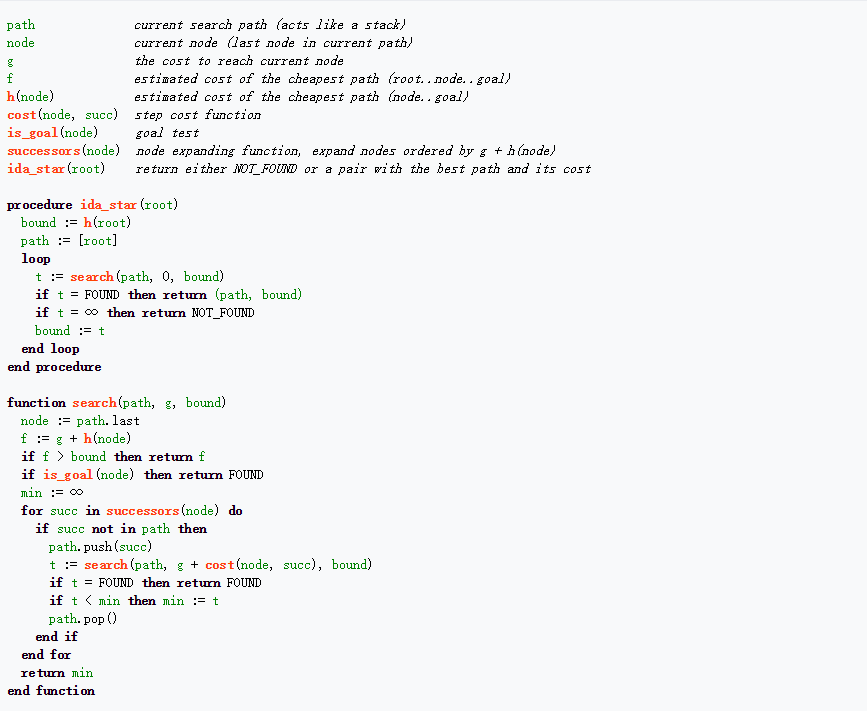
\includegraphics[width=17.3cm]{Pic/code}
\end{figure}
\section{Tasks}



\begin{itemize}
	\item Please solve 15-Puzzle problem by using IDA* (Python or C++). You can use one of the two commonly used heuristic functions: h1 = the number of misplaced tiles. h2 = the sum of the distances of the tiles from their goal positions.
	\item Here are 4 test cases for you to verify your algorithm correctness. You can also play this game (\texttt{15puzzle.zip}) for more information.
	\begin{figure}[ht]
	\centering
	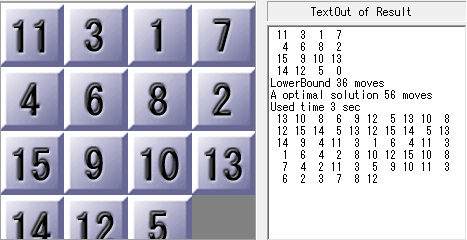
\includegraphics[width=8cm]{Pic/case1}
	\quad
	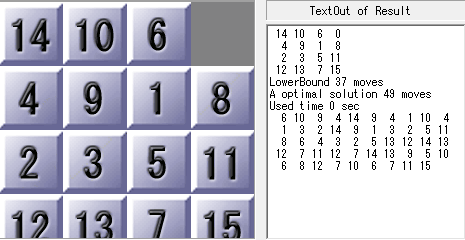
\includegraphics[width=8cm]{Pic/case2}
	\\
	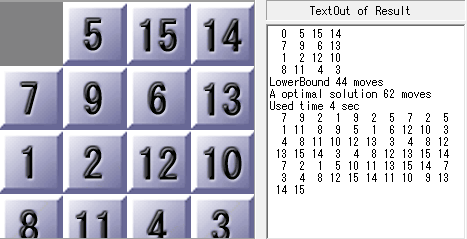
\includegraphics[width=8cm]{Pic/case3}
	\quad
	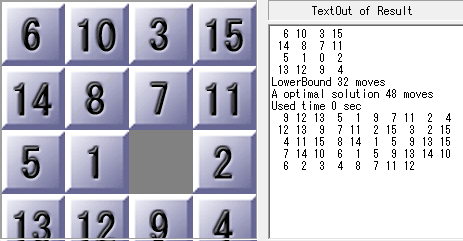
\includegraphics[width=8cm]{Pic/case4}
	
	\end{figure}
	\item Please send \texttt{E02\_YourNumber.pdf} to \texttt{ai\_201901@foxmail.com}, you can certainly use \texttt{E02\_15puzzle.tex} as the \LaTeX template.
\end{itemize}


\section{Codes}
\lstset{language=C++}
%%\lstset{language=Python}
\begin{lstlisting}

\end{lstlisting}
\section{Results}
\begin{figure}
\centering
%%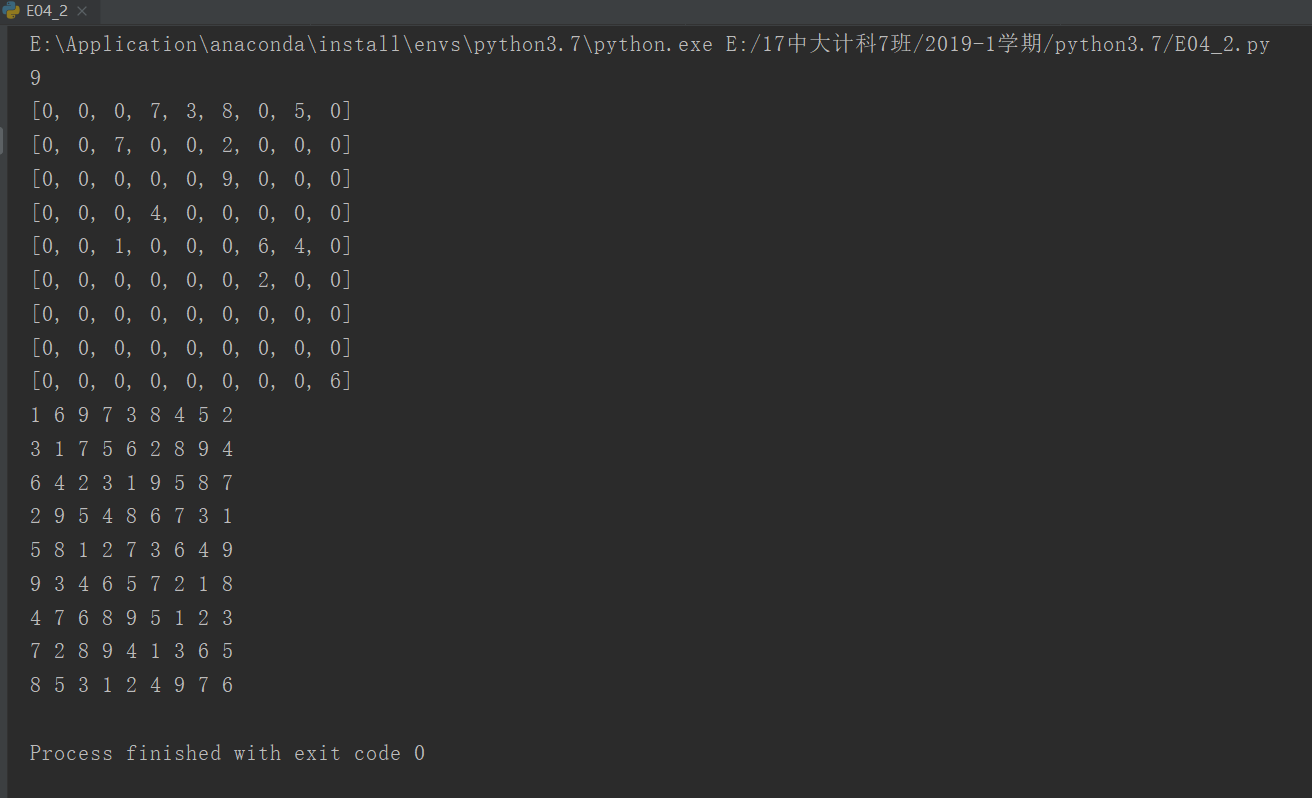
\includegraphics[width=15cm]{result.png}
\end{figure}


%\clearpage
%\bibliography{E:/Papers/LiuLab}
%\bibliographystyle{apalike}
\end{document}
